\documentclass[main]{subfiles}
\begin{document}
\section{グリッド}
\begin{table}[H]
  \centering
  \caption{Parameters}
  \begin{tabular}{lcccc}
		\hline
    \textbf{Name} & \textbf{Min} & \textbf{Max} & \textbf{Resolution} & \textbf{Unit} \\ \hline \hline
    icp, x        & -0.60 & 0.60 & * & [m] \\
    icp, y        & -0.60 & 0.60 & * & [m] \\
    swing foot, x & -0.25 & 0.25 & * & [m] \\
    swing foot, y &  0.20 & 0.50 & * & [m] \\
    \hline
  \end{tabular}
\end{table}
足の頂点\\
+0.115, +0.065\\
+0.115, -0.065\\
-0.115, -0.065\\
-0.115, +0.065\\
\begin{figure}[H]
  \centering
  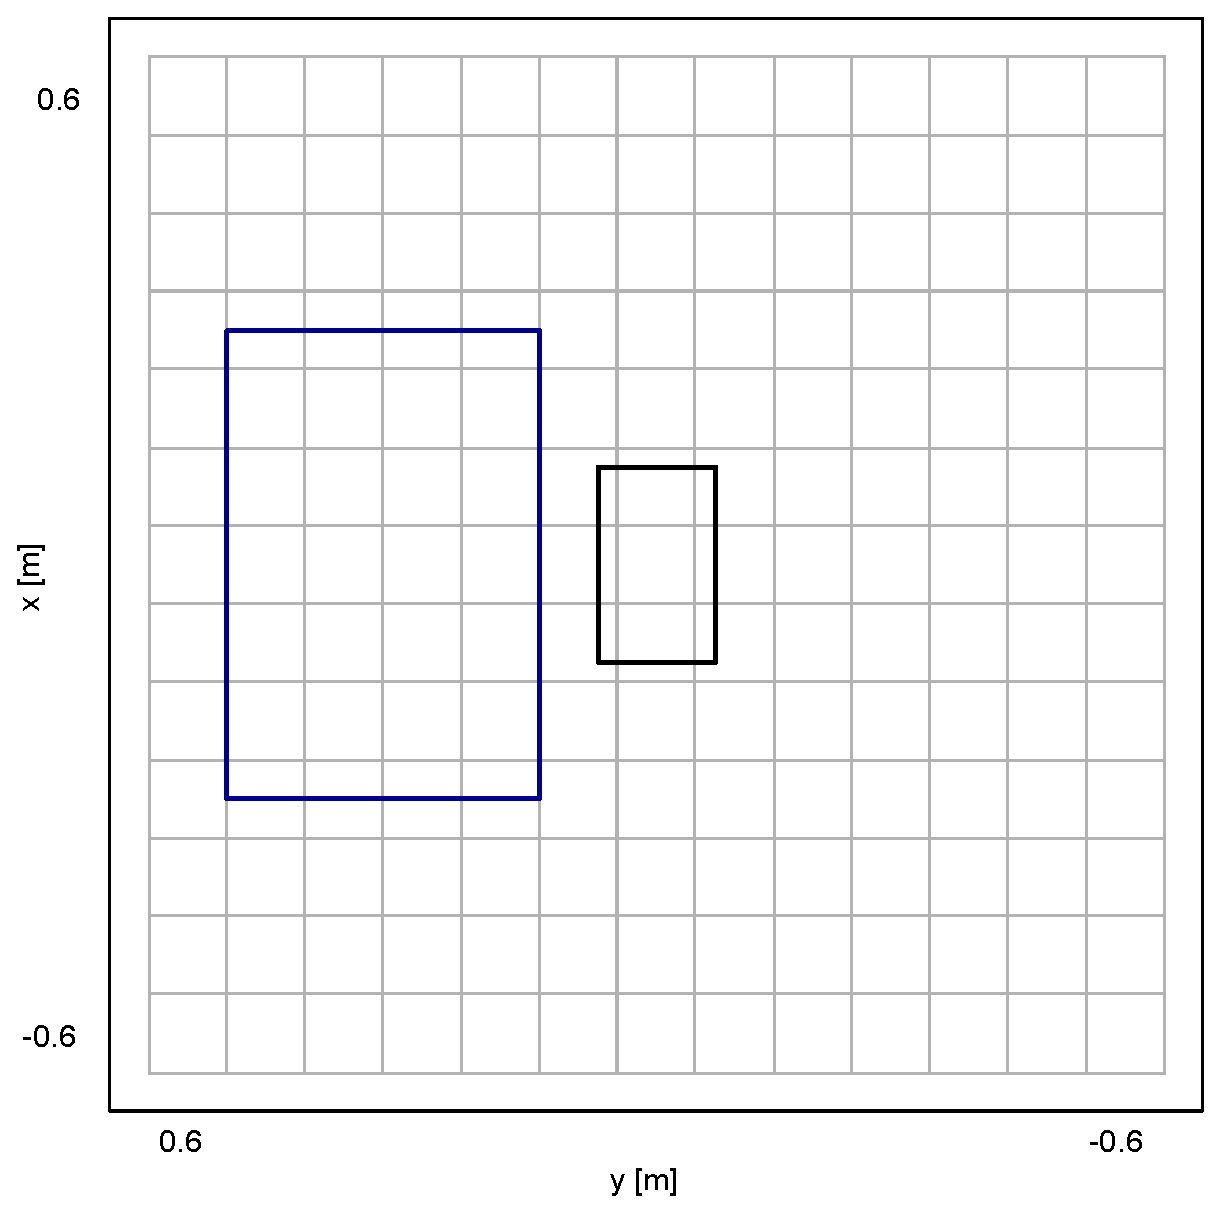
\includegraphics[width = 100 mm]{graph/grid/0.1.eps}
\end{figure}
\begin{figure}[H]
  \centering
  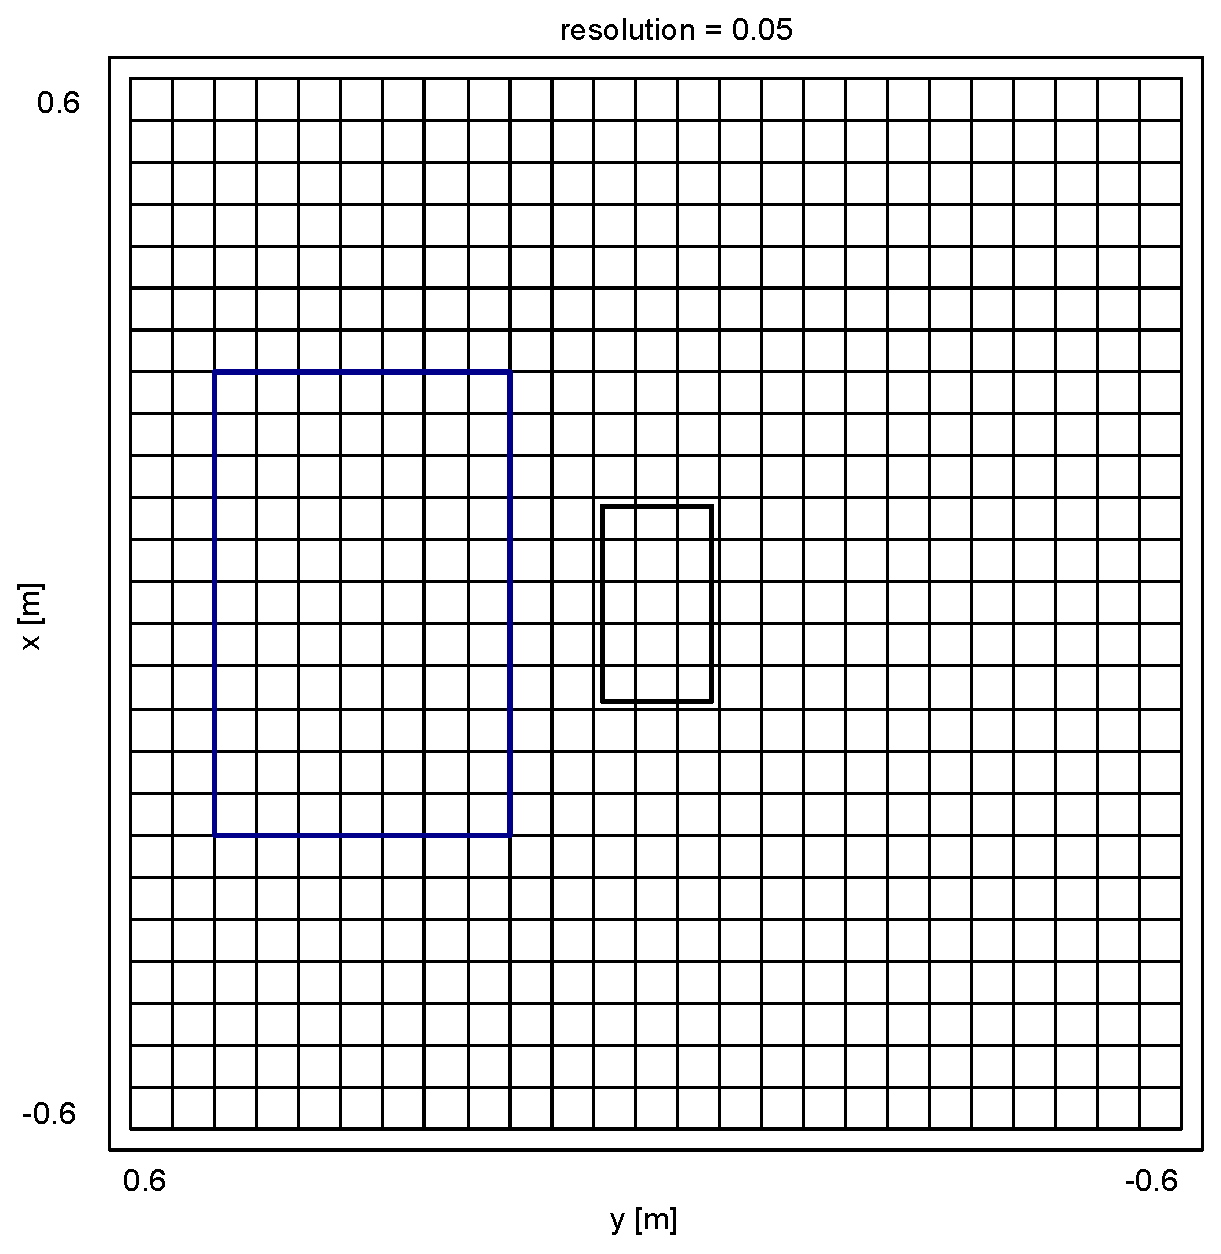
\includegraphics[width = 100 mm]{graph/grid/0.05.eps}
\end{figure}
\begin{figure}[H]
  \centering
  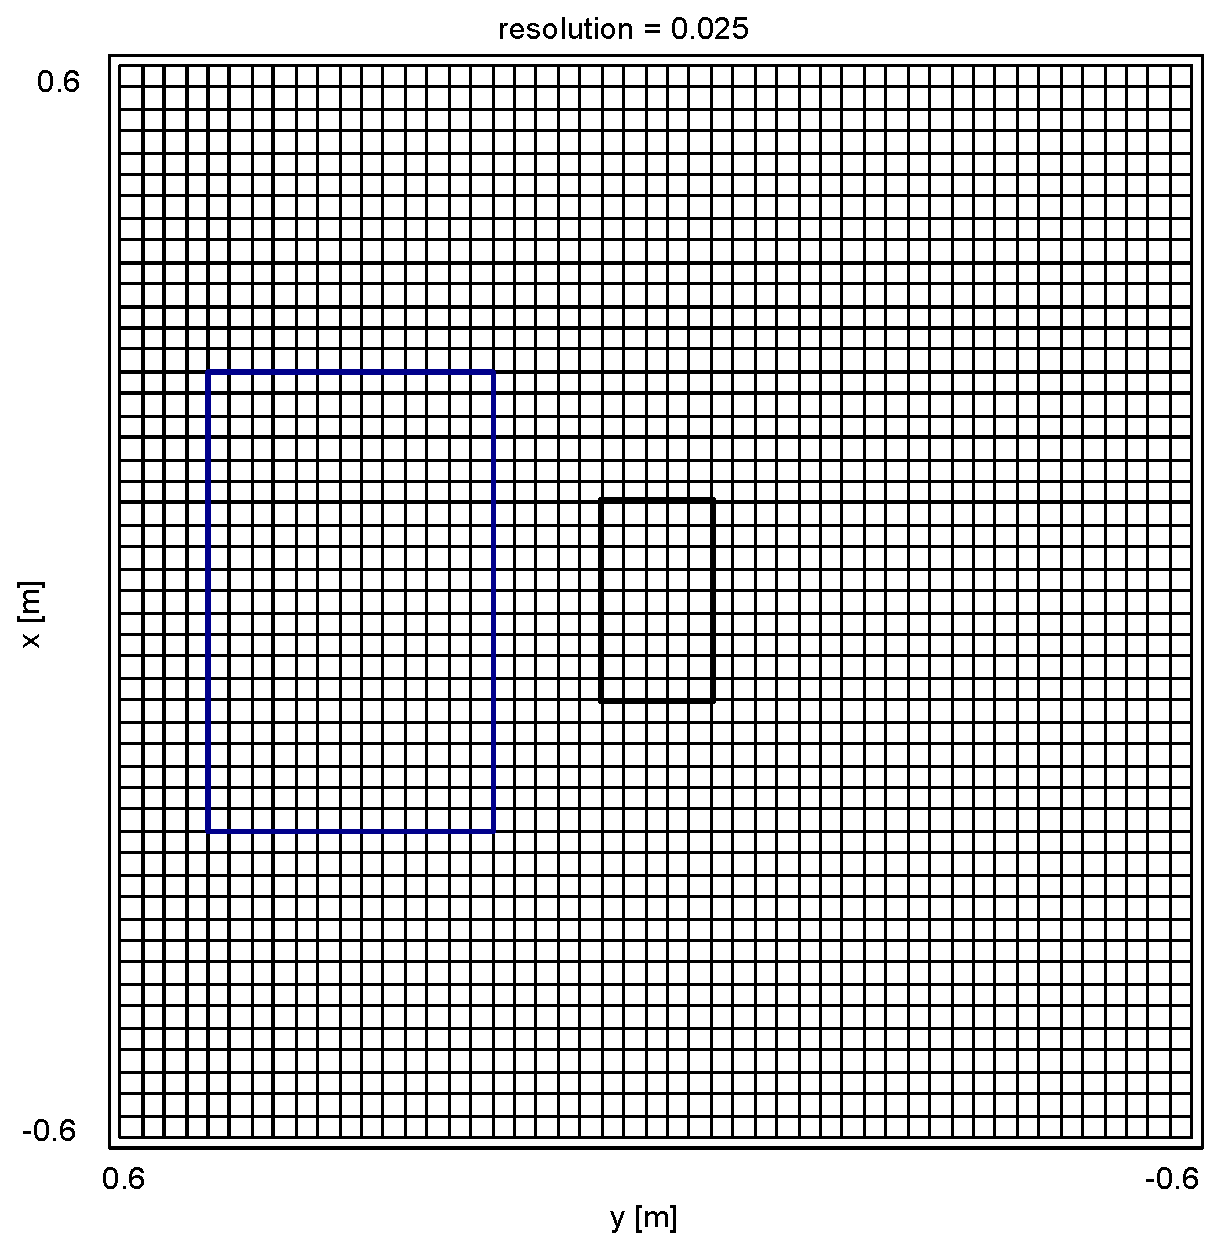
\includegraphics[width = 100 mm]{graph/grid/0.025.eps}
\end{figure}
%-----------------------------------------------------------------------------%
\end{document}